\section{How to improve security in identity federations}
%Security in identity federations involves data integrity, which is said to be true when
%the federations entities can share trusted metadata between each other. 
%The metadata is trusted when the entities in the federation can identify each other with the help of 
%certificates within the metadata file.

%Messages sent between entities depend on the data integrity being held.
This section evaluates the security in identity federations with the first question from problem area in mind.

Messages sent between entities within the identity federations depends on the data integrity being held.
However, the most difficult part is setting up SAML's initial trust relationship between entities, the first exchanging of keys.
The SAML metadata document says \emph{"...to aid in establishing trust in the accuracy and legitimacy of metadata,
including use of XML signatures, TLS or SSL server authentication, and DNS signatures.
Regardless of the mechanism(s) used, relying parties SHOULD have some means by which to establish trust in metadata information
before relying on it."} \cite[p.~29]{pdf:oasis-open-metadata}.

With that said, after the first certificate exchange has been made a trust relationship is built and the data integrity is up and running. 
The question is, how can the first certificate exchange be made securely? 
One solution might be a third party, a CA or the use of DNSSEC or maybe both to validates that the certificates is the right ones.
Another one could be to use Pretty Good Privacy (PGP)  \cite{rfc:2440} to sign or encrypt the certificate before transmission.
With this solution, the soon to be certificate receiver first sends a PGP encrypted message containing its contact
information to the certificate sender, that decrypts the message. Finds out the receivers phonenumber and calls him or her
to confirm the message sender and key used in the PGP message.
When it is confirmed that it came from the receiver, the certificate sender sends the certificate to the receiver.

Furthermore, the communication standard described in SAML could be more strict.
That involves the first certificate exchange just mentioned. 
Another example is the certificate itself, the SAML bindings document says  
that the bindings which use TLS or SSL has to authenticate clients using X.509 certificate \cite[p.~8]{pdf:oasis-open-bindings} and the metadata profile document says
\emph{"In the case of an X.509 certificate, there are no requirements as to the content of the certificate apart from the requirement 
that it contain the appropriate public key. 
Specifically, the certificate may be expired, not yet valid, carry critical or non-critical extensions or usage flags, and contain 
any subject or issuer. 
The use of the certificate structure is merely a matter of notational convenience to communicate a key and has no semantics in this 
profile apart from that. 
However, it is RECOMMENDED that certificates be unexpired."} \cite[p.~11]{pdf:oasis-open-metadata-profile}. 

By changing the SAML documents guidelines in general to be less open for interpretation it could improve the security. 
For example to not recommend that the certificates has not expired, but express that they should or must not be expired. 
Moreover, it is a vulnerability that the metadata file can contain expired certificates.

Without stricter guidelines an online check of the certificate could also be a solution to the expired certificate problem. 
The Online Certificate Status Protocol (OCSP) \cite{rfc:6277} could be used to perform this online check.

\section{How to combine identity federations and DANE}
As stated earlier it's possible to divide federations into two categories, those with a federation operator and those without.
In the analysis that has been done the solution with a federation operator is the most probable and viable setup in the long run, it's basically much easier to scale, both technically and non-technically.
It's with this configuration in mind the following evaluation has been made.

%TODO: (1) Kontrollera att det finns information om båda kategorierna av federationer.
%TODO: (2) Kontrollera att analys är gjord och att det verkligen är varianten med en FO som är mest trolig.

With a federation operator publishing all the metadata about all service providers, identity providers and other entities how do the trusting entites rely on the federation operator?
Is it the correct federation operator the trusting entities connect to or is it someone trying to "impersonate" the role of the federation operator as a man-in-the-middle attack.

As of now the trust must be made in some out-of-band way e.g. a simple download of the federation operator's certificate and then confirm it's the correct one via telephone, email communcation between administrators or meet in person.
This is not very practical when the federation grows bigger with tenths or hundreds of service- and identity providers or is it the only way?
\subsection{How to publish certificates}
\subsubsection{SAML2 certificate as CERT resource record}
\label{subsec:saml2-certificate-as-tlsa}
The first solution that comes into mind is that it might be possible to publish the federation operator's certificate in the Domain Name System and more specifically as a CERT RR\cite{rfc:4398}.
This would mean that when a requesting entity (service provider, identity provider or any other entity) needs to update the metadata about all other entities it connects to the federation operator and downloads the metadata.
At the same time the requesting entity sends out a DNS lookup (with DNSSEC active) for a corresponding CERT RR.
When both the metadata and the CERT RR is retrieved, a comparison can be made and confirm or dismiss the validity of the metadata.
This is done after step 3 and 4 in figure \ref{ch4:saml2certsascertrr}.

A problem that still exists with this approach is how will each entity transmit metadata about itself to the federation operator and how will the metadata be validated by the federation operator (Step 1 and 2 in figure \ref{ch4:saml2certsascertrr}).
To keep building on the same solution each entity would have to publish respective certificate as a CERT RR themselves in their own domain zone.
They would also need to sign their own metadata which is not the case in current standards. 
Now the initial upload of metadata from an entity to the federation operator could be intitated, perhaps through a web interface, with or without some "Pretty Good Privacy" (PGP) solution e.g. OpenPGP\cite{rfc:2440}.
% TODO: Add use cases from registry->registrar in DNS and how it is used their.
The federation operator then fetches the metadata as well as the corresponding CERT RR from the entity and if it's the correct signature on it the federation operator can publish it with the metadata from all other entities.
Within one cache interval all entities will now fetch the complete updated metadata from the federation operator.

\begin{figure}[ht]
\begin{center}
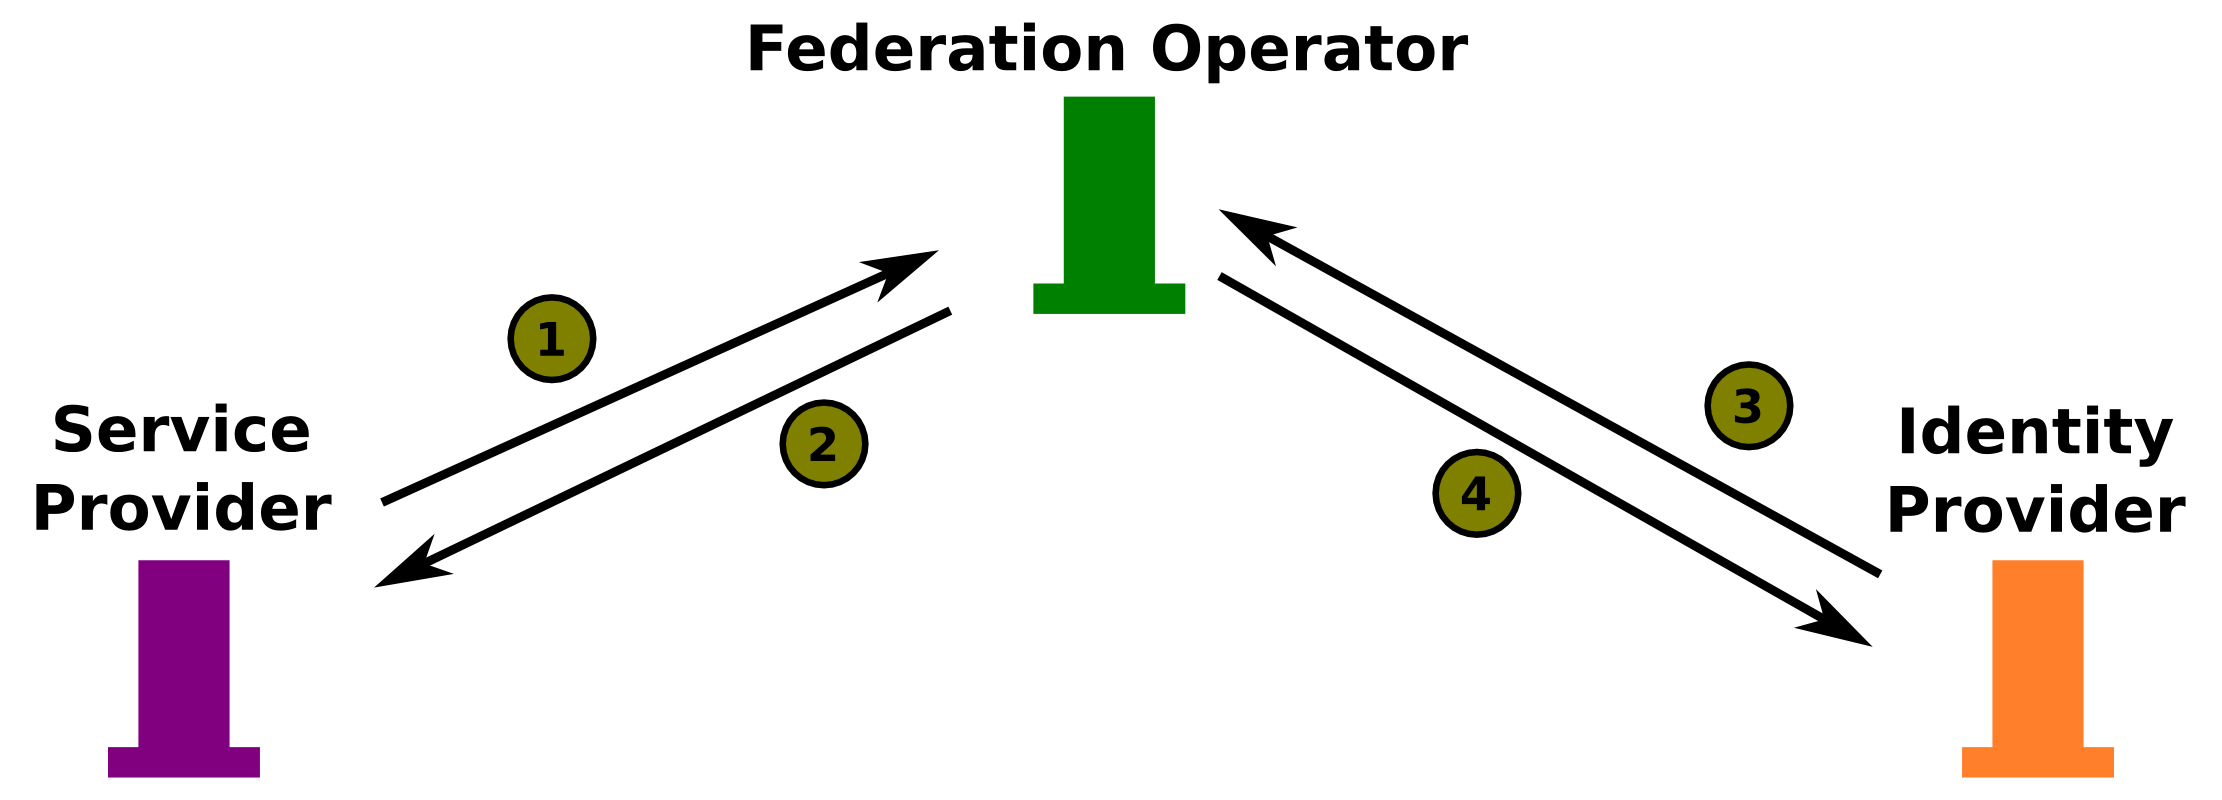
\includegraphics[scale=1]{Figures/saml2certsascertrr.png}
\end{center}
\caption{A complete cycle of transmitting metadata securely from the Service provider to the Identity provider via a federation operator.
Step 1, the service provider initiate an update of metadata.
Step 2, the federation operator requests the metadata from some well known location.
Step 3, the identity provider updates the local metadata cache when the cache timer has expired by requesting new metadata from the federation operator.
Step 4, the federation operator respond with the new metadata.
After each response that includes a certificate in some form another request is made to the domain name system for CERT RRs to be able to validate the original certificate.
\label{ch4:saml2certsascertrr}}
\end{figure}


% TODO: What is a cache interval?
% TODO: What is a domain zone?

New questions arises here, is it practical to store SAML2 certificates in the Domain Name System as a CERT RR 
or are there better alternatives?
The second question that comes to mind is more related to DANE.
If CERT RRs is used as stated above it would require DNSSEC otherwise its value would be of no use.
Is it not possible to just use the TLSA RR with TLS certificates as it is and not introduce another layer that CERT RRs would become within the same system (DNS and DNSSEC)?

\subsubsection{Only use TLS (with TLSA RR)}
\label{subsec:only-tlsa-rr-with-tls}
Let's start with the question would it be enough within identity federations to only use TLS with TLSA and not to publish any SAML certificates?

The solution is already at the point where all entities within a federation needs to sign their own zone with DNSSEC as an underlying infrastructure.
Instead of publishing SAML2 certificates in the Domain Name System it might be possible to just use TLS with TLSA RRs and deem that all the information communicated between any two entities is valid as long as it's over TLS that has been established with TLSA RRs procedures.

This would mean that when a new entity, let's say a service provider, joins a federation the service provider must send its metadata to the federation operator.
As an example the administrator for the service provider might visit a webpage over HTTPS (with validity check for TLSA RR) to initiate the transfer of metadata, step 1 in figure \ref{ch4:onlyUseTLS}.
The federation operator then opens a new connection over HTTPS (with validity check for TLSA RR) for the metadata from the service provider, step 2 in figure \ref{ch4:onlyUseTLS}.
This request, from the federation operator back to the service provider, that initiated the communication the first time is to make sure that the metadata that is fetched is from the right service provider. 
When the metadata is recieved the federation operator can publish it with the metadata for all other entities, step 3 in \ref{ch4:onlyUseTLS}

\begin{figure}[ht]
\begin{center}
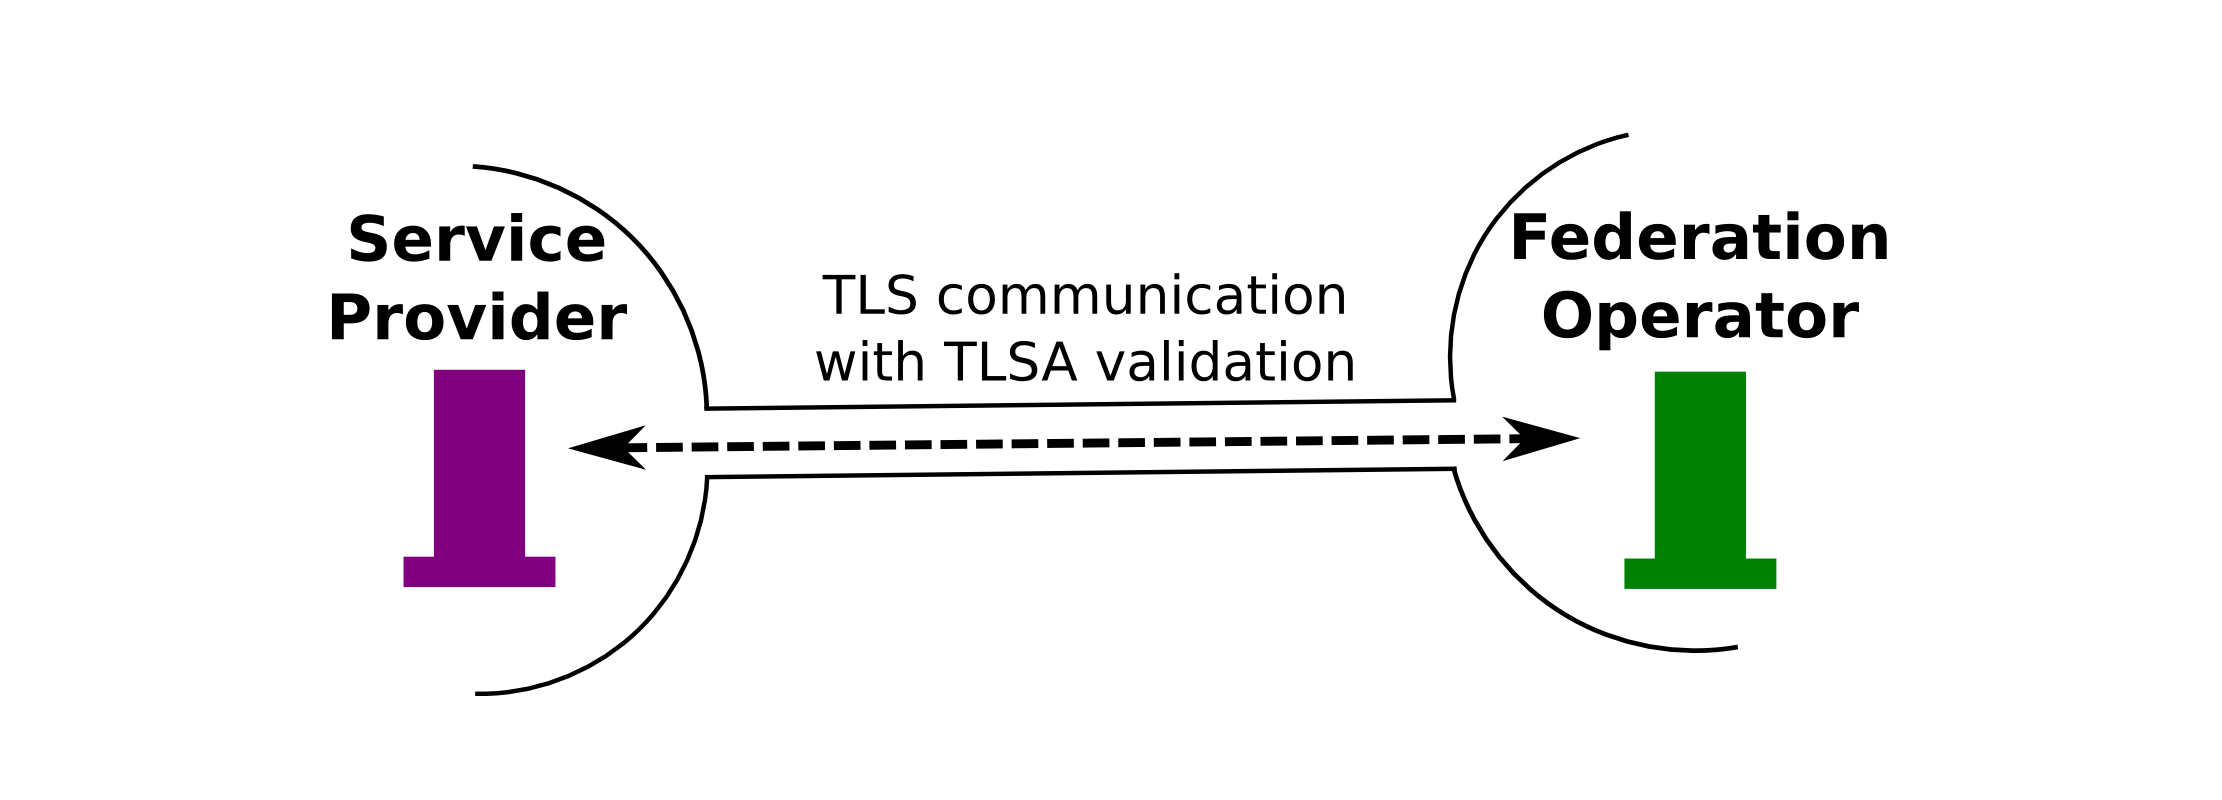
\includegraphics[scale=1]{Figures/onlyUseTLS.png}
\end{center}
\caption{A simple procedure to establish first time communication with a new member in an identity federation.
\label{ch4:onlyUseTLS}}
\end{figure}

%
% TODO: What is metadata?
% TODO: What is an entity?

\subsubsection{Publishing SAML2 certificate as CERT RR, is it viable?}
\label{subsec:saml2-certs-in-cert-rr}
Earlier in this chapter the question arose if it is practical to store SAML2 certificates in the Domain Name System.
Due to time constraints this is out of scope of this report and further investigations has to be done in this area.
For further discussions in this report it's assumed that it's a viable solution to store SAML2 certificates in the Domain Name System as CERT RRs.

\subsubsection{Using the best of two worlds}
It's often the simple solution that is the best one but would it be worth it to use TLSA validated connection for the HTTPS communication together with the SAML2 certificates in CERT RRs as explained in earlier sections?

To simplify the view an argument could be made that the validity check on the SAML2 certficate downloaded over the HTTPS secure channel and then verified against the CERT RR is just another safety check within the same "layer" as the secure channel was established in.
The reason for this is that the TLS connection is validated first with information from the DNSSEC infrastructure, when requesting the TLSA RR.
The second validation is made depending on the TLSA RR information and local policies, it confirms that the TLS server certificate chain is to be trusted or not.
The third validation would be when the SAML2 certificate is compared against the CERT RR available within the DNSSEC infrastructure.

As noted the first and the third validation are both trusting the DNSSEC infrastructure, and therefore the combination of both using TLS with TLSA and SAML2 certificate with CERT RRs would at first glance not add any extra benefits.
Though under some circumstances someone might be able to hack into a webserver for some entity and change the certificate used for SAML2 signing.
Common production setup is to put the DNS servers on seperate instances than the webserver and if only the webserver is compromised the third validation check against the CERT RR would in this case fail.
So in the end the question boils down to if the communication is secure to the correct host, is this enough to trust everything that the host sends?

\begin{figure}[ht]
\begin{center}
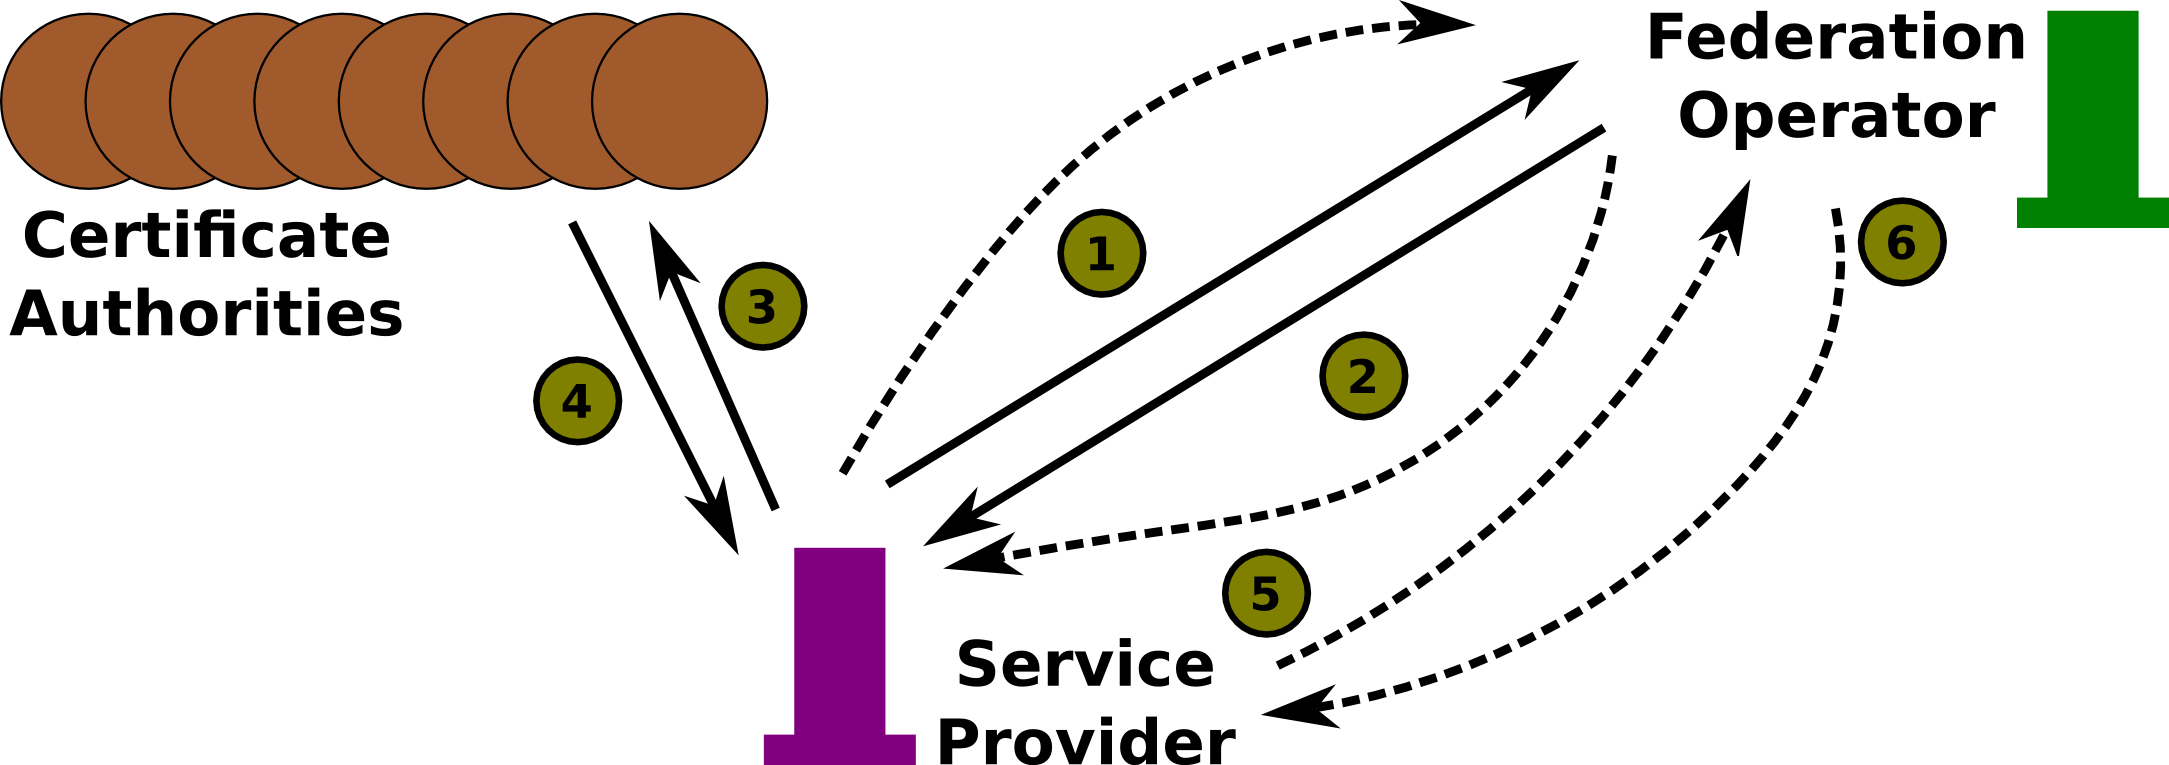
\includegraphics[scale=1]{Figures/bestOfTwoWorlds.png}
\end{center}
\caption{Three validation checks divided into 6 different requests or responses.
Step 1 and 2 is the initial communication when the TLS communication is established with TLSA.
Step 3 and 4 is when local policy demands that the certificate recieved within the metadata has to be validated that it chains to a CA.
Step 5 and 6 is the last validation step when the Service Provider requests corresponding CERT reosource records from the federation operator and checks that the certificate used to sign the metadata is available as a CERT RR.
\label{ch4:bestOfTwoWorlds}}
\end{figure}

%\subsection{The matching dilemma}
\subsection{How to locate the correct certificate in DNS}
\label{subsec:matching-dilemma}
The last section was about how to distribute the certificate within the Domain Name System and if it's necessary or not.
The CERT RR is mentioned as a possible solution and there might be several other solutions as well.
If it's decided upon that a TLSA validated TLS connection is not enough to trust the data that is being sent the SAML2 certificates must be published as well in the Domain Name System.
With a single or just a few certificates that signs several metadata files for the federation operator it's relatively easy to publish the certificates in the Domain Name System and fetch all certificates based on the domain or subdomain.
Though it would put an unwanted limit that the federation operator is only allowed to use a few certificates per DNS zone.
Of course it would work with several hundred certificates but it wouldn't be a very good solution.
This is because each time some entity would check if one specific certificate is the correct one the requesting entity would have to download all certificates through the Domain Name System and then one by one try to match them against the certificate used in the fetched metadata file.

This means that somekind of general algorithm or solution is required to locate the correct certificate published in the Domain Name System when an entity recieves a signed metadata file.
One way of doing this might be with the "Dynamic Delegation Discovery System (DDDS)"\cite{rfc:3401,rfc:3402,rfc:3403,rfc:3404} and the NAPTR resource record\cite{rfc:3403}.
Exactly how this could be done is out of the scope of this report.

The main issue and possible solution in this section was originally introduced by Leif Johansson (SUNET).

\section{How DANE can be implemented in Shibboleth} 
DANE as a technology is on the way to becoming a standard within TLS communication and sooner or later also for S/MIME.
There is not even a draft available for the use together with certificates concerning other usages than those, therefore there is no way to "implement" DANE for Shibboleth (concerning the SAML2 certificates that is).
% What has been implemented is more of a proof-of-concept for future reference if/when there is a standard available.

%The implementation has been solely done on the Identity provider to keep the focus on one implementation instead of trying to implement it on both the service provider and identity provider software.
%Main reason for this has beeen time constraints.

As stated in previous chapter the software for the identity provider part is written in Java.
It has several extension points where the functionality of different parts can be extended.
Due to the number of extension points some reading had to be done to figure out exactly which extension type was best suited for the purpose of a DANE extension.

First possibility was the "Metadata Provider" extension point.
The "Metadata Provider" extension point is the part in the identity provider that control the retrieval of metadata.
An example to this is the "File Backed HTTP Metadata Provider", it basically fetches the metadata from an URL and stores a cache locally on the server.

The second extension possiblity was a "Metadata Filter" extension.
An example to this one is the "Required Valid Until" which checks some arguments in the retrieved metadata if the metadata has a "valid until" argument set not to far in to the future.

Third and fourth extension type that might have worked for the purpose of a DANE implementation are the "Security Policy" and "Security Policy Rule" extension types.
Both these relates to security concerning individual messages between service and identity providers and not the initial loading of metadata, which in the end ruled these out as viable solutions.

The solution finally chosen to be implemented was a trust engine extension.
A trust engine is a part of Shibboleth that processes either metadata or other messages to validate it or dismiss the message.
An example trust engine is the "Static Explicit Key Signature Trust Engine" that takes one or more certificates compares it with signed metadata and confirms that the signature is the right one. 

% TODO: More research into this? Perhaps we will give an answer to this that is enough.

%\section{Temporary section}
%EVALUATION This is where you put the spotlight on your solution's strengths and
%weaknesses. An evaluation must be made of the methods/theory applied and the validity
%and reliability of the data. You should describe the most interesting results of your work in a
%results section. Remember that less important but complementary results can to advantage
%be placed in appendices. A rule of thumb is that all results that you use in your analysis and
%in your conclusions should be reported in the Evaluation chapter and the rest reported in
%appendices.

